
\chapter{Diseño de SIDManager} \label{disenyo}

\section{Modelo de los documentos}
\label{subsec:document-architecture}
Para comprender bien las tablas de la base de datos que vamos a utilizar, cabe destacar que se ha empleado una base de datos de la empresa Santander. Al ser una base de datos de una entidad bancaria, no se pueden mostrar todas las entidades de esta base de datos por motivos de seguridad. Es por este motivo que aquí únicamente hablaremos de las entidades directamente relacionadas con la aplicación, que son dos. La primera ya existía antes de crear la aplicación y se llamaba Documents (Documentos) y la segunda se creó durante el desarrollo de la aplicación SIDManager; su nombre es ClientUser (Usuario Cliente o simplemente usuario). 

En caso de querer saber más sobre la base de datos, consulte el esquema del anexo \ref{fig:BD-scheme}.

A lo largo del siguiente capítulo se hablará mucho de los documentos; por ello, es necesario explicar bien a qué queremos decir cuando hablamos de estos. Esta aplicación ha sido creada, como se ha dicho anteriormente, con el fin de confirmar si los documentos están guardados correctamente, pero estos pueden contener información sensible a la cual no debemos acceder. Es por ello que, inclusive, los metadatos de este documento están restringidos. Es por ello que debemos mostrar la mínima información posible al usuario sobre el documento, pero que sepa que este está correctamente guardado. Para ello, en la aplicación, los documentos tienen 5 apartados:
\begin{enumerate}
    \item client\_app\_id:
    identificador numérico de la aplicacion del cliente, es el identificador que tiene la aplicación que ha creado el documento, es decir, si en la empresa hay 3 aplicaciones como OutSystem, Vue y Java cada una de estas aplicaciones tendría un identificador (1, 2 y 3). Por tanto con este dato sabemos en que aplicación se ha creado el documento. Podríamos definir cliente como la aplicación donde ese crea. Este identificador es repetible ya que dos documentos pueden ser creados por la misma aplicación.


    \item client\_doc\_id:
    identificador numérico del documento del cliente, es el identificador que la aplicación le ha asignado al documento. Como las aplicaciones no pueden ni deben acceder a los documentos de otras, este identificador se puede repetir de una aplicación a otra. Es decir, podría haber el primer documento creado por Java y el primer documento creado por OutSystem. Para resumir este identificador es repetible ya que dos documentos pueden tener asignados el mismo identificador por aplicaciones distintas.


    \item provider\_id: identificador numérico del proveedor, es el identificador asignado a las empresas que a partir del documento en un formato de datos basado en texto, se encargan de procesarlo y convertirlo a un formato adaptado a la impresión y enviarlo en formato físico y digital.

    \item sent\_at:
    Este campo corresponde a la fecha y hora a la que el documento fue mandado a a la empresa que se encarga de procesarlo (proveedor) en formato timestamp (aaaa/mm/dd hh:mm:ss).
   
    \item received\_at: 
    Este campo corresponde a la fecha y hora a la que el documento fue recibido en la base de datos de la propia empresa, es decir, con este campo podemos saber si un documento está correctamente guardado en la base de datos y no se ha perdido (ya que los proveedores pueden cometer el error de no enviar de vuelta el documento). Tiene el mismo formato que sent\_at.

\end{enumerate}

Veamos un ejemplo de cómo se vería un documento en la aplicación SIDManager para mayor comprensión de estos. En este apartado se van a hacer varios supuestos para entender qué significa cada campo del documento tal y como vemos en la tabla \ref{table:documentModel}.

\begin{table}
    \caption{Modelo de los documentos}
    \label{table:documentModel}
    \begin{center}
    \begin{tabularx}{\textwidth}{|l|X|X|}
    \hline
    \textbf{Nombre} & \textbf{Ejemplo de Contenido} & \textbf{Interpretación} \\
    \hline
    Client app id & 20 & Puede indicar que ha sido creada por la aplicación de Java (si Java es la aplicación número 20) \\
    \hline
    Client doc id & 12385823 & Quiere decir que de todos los documentos creados con java es el número 12385823 \\
    \hline
    Provider id & \texttt{jiehw72ih4r94yir9712} & Empresa que procesa los documentos (ej. Accenture) \\
    \hline
    Sent at & \texttt{2023-08-07 22:02:12} & Fecha y hora de envío del documento al proveedor \\
    \hline
    Received at & Not received & Documento aún no recibido por el proveedor (representado como \texttt{null} en la base de datos) \\
    \hline
    \end{tabularx}
    \end{center}
\end{table}


\section{Modelo de los usuarios}
\label{subsec:user-architecture}

A lo largo del siguiente capítulo se hablará en múltiples ocasiones sobre los usuarios, por lo que es necesario explicar con detalle a qué nos referimos cuando mencionamos este concepto dentro del sistema.

Los usuarios en la aplicación representan a las personas que interactúan con el sistema, ya sea para acceder a sus funcionalidades o para gestionar información. Cada usuario está debidamente registrado en la base de datos con ciertos atributos que permiten su autenticación y gestión dentro de la plataforma. 

Para garantizar la seguridad y la correcta administración de los accesos, cada usuario en la aplicación se define mediante los siguientes apartados:

\begin{enumerate}
    \item Email:  
    Es la dirección de correo electrónico del usuario. Se utiliza como identificador único del usuario en el sistema, permitiendo que cada usuario acceda con sus credenciales y reciba notificaciones o confirmaciones por correo.

    \item Password:  
    Contraseña asociada a la cuenta del usuario. Por razones de seguridad, la contraseña no se almacena en texto plano, sino que se codifica mediante un algoritmo de cifrado seguro (como se explicará en capítulos posteriores). En la base de datos se almacena la versión encriptada de la contraseña, lo que impide que sea visible en su formato original.

    \item Code:  
    Código único generado para cada usuario en el momento de su registro. Este código será utilizado en dos situaciones clave, a la hora de confirmar el registro y al recuperar la contraseña.
    Cuando un usuario se registra, se le envía un correo con este código para verificar su identidad y confirmar la cuenta.
    Si un usuario olvida su contraseña, este código se usa para permitirle restablecerla de manera segura.

    
    \item Status:  
    Representa el estado actual de la cuenta del usuario. Puede tener dos valores, 0 o 1.
    Cuando el valor de status es 0 significa que el usuario ha sido creado en la base de datos, pero aún no ha confirmado su correo electrónico.
    Sin embargo cuando el valor de status es 1 quiere decir que el usuario ha completado el proceso de confirmación y su cuenta está activa.

    
    \item Creation Date:  
    Fecha y hora en la que el usuario se registró en la plataforma. 

    \item Confirmation Date:  
    Fecha y hora en la que el usuario confirmó su cuenta mediante el código de verificación enviado a su correo. Si este campo es nulo (null), significa que el usuario aún no ha validado su dirección de correo electrónico y, por lo tanto, no tiene acceso completo a la plataforma.

\end{enumerate}

Para una mejor comprensión de cómo se almacenan los usuarios en la base de datos, se puede consultar un ejemplo de cómo se vería un usuario en el sistema en la tabla \ref{table:userModel}.

\begin{table}
    \caption{ Modelo de los usuarios}
    \label{table:userModel}
    \begin{tabularx}{\textwidth}{|l|X|X|}
    \hline
    \textbf{Nombre} & \textbf{Ejemplo de Contenido} & \textbf{Interpretación} \\
    \hline
    Email & \texttt{elias@gmail.com} & Correo con el que el usuario se registró en la plataforma \\
    \hline
    Password & \texttt{\$2a\$10\$HnIEMbmEeayF5fuz 4LQH0OGWBPifFDX5/WMahhl S5AogsGK1Zh7tG} & Contraseña almacenada encriptada con BCrypt para mayor seguridad \\
    \hline
    Code & \texttt{CAWUxr2Gz4nGcWkOsLyGysh GDhbOtL} & Código único del usuario, utilizado para la validación de la cuenta \\
    \hline
    Status & \texttt{0} & Indica que la cuenta ha sido creada pero aún no confirmada \\
    \hline
    Creation Date & \texttt{2024-08-26 16:50:09.0} & Fecha y hora en que el usuario se registró en la plataforma \\
    \hline
    Confirmation Date & \texttt{null} & Indica que el usuario aún no ha validado su cuenta \\
    \hline
    \end{tabularx}
\end{table}



\section{Descripción de las capas de la aplicación}

En esta sección se describe la arquitectura seleccionada para el desarrollo del sistema, destacando la división entre el frontend y el backend, y cómo estos componentes interactúan para ofrecer una experiencia fluida al usuario. La arquitectura sigue un patrón típico de aplicaciones web basado en capas, un ejemplo de esto podría ser la arquitectura modelo-vista-controlador (MVC) explicada en el artículo \textcite{MVC}.

La arquitectura seleccionada se basa en el framework Spring Boot para el backend y Thymeleaf para el frontend. Este enfoque garantiza una integración robusta entre la lógica de negocio y las interfaces de usuario.

El usuario interactúa con la aplicación a través de las interfaces de frontend desarrolladas con Thymeleaf, un motor de plantillas que permite generar dinámicamente las vistas en función de los datos obtenidos desde el backend. Estas interfaces envían y reciben peticiones HTTP (HTTP requests), que son gestionadas por los controladores en el backend.

La Figura \ref{fig:arquitecture_SIDManager} muestra un esquema de la arquitectura seleccionada, donde se representa la interacción entre las capas y cómo se comunican entre sí. La información detallada sobre cada capa es la siguiente:

\begin{figure}
    \centering
    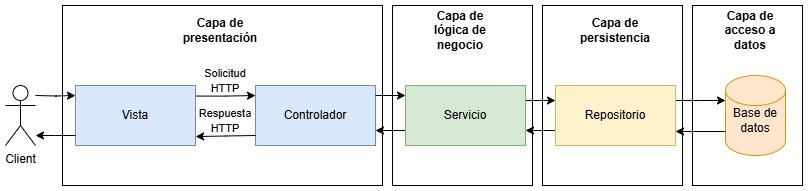
\includegraphics[width=0.95\linewidth]{imagenes/scheme/arquitectura-SIDManager.jpg}
    \caption{Arquitectura de las capas aplicación SIDManager}
    \label{fig:arquitecture_SIDManager}
\end{figure}

\begin{enumerate}
    \item Capa de presentación:
    La capa de presentación es la encargada de manejar la interfaz de usuario y las interacciones del usuario, presentando información a los usuarios y capturando su entrada.
    En este proyecto contiene dos componentes en esta capa, la vista y el controlador.
    Por un lado el cliente accede a las interfaces visuales, las cuales están diseñadas con Thymeleaf para garantizar una generación dinámica y eficiente de las vistas (views). Este motor de plantillas permite incluir datos provenientes del back-end directamente en las páginas HTML, facilitando la comunicación entre ambas capas.
    Por otro lado los controladores (controllers) son responsables de gestionar las peticiones HTTP provenientes del front-end. Estos se encargan de procesar la solicitud y delegar la lógica de negocio al siguiente nivel, los servicios (services). En otras palabras, son conectores que dirigen las peticiones del usuario a los servicios correspondientes sin modificar ni hacer operaciones de lógica de negocio.

    \item Capa de negocio:
    Esta capa es la encargada de implementar la funcionalidad principal y las reglas que impulsan los procesos y operaciones del negocio.
    En la aplicación, está capa esta definida en los servicios, que se encargan de realizar las transformaciones necesarias sobre los datos y delegan las operaciones de almacenamiento o consulta al repositorio.

    \item Capa de persistencia:
    La función principal de esta capa es manejar el almacenamiento y recuperación de datos de bases de datos.
    En este proyecto contiene dos componentes en esta capa, del repositorio y el modelo.
    Por un lado, el repositorio (repository) utiliza JPA (Java Persistence API) y se conecta con la base de datos para realizar operaciones CRUD (Crear, Leer, Actualizar, Eliminar). 
    Por otro lado, el modelo (model) está representado por los datos manejados por la aplicación mediante entidades JPA. Estos modelos mapean las tablas de la base de datos, permitiendo que la lógica de negocio interactúe con ellas de forma directa.
    Esta capa abstrae los detalles de implementación de la base de datos, permitiendo una interacción más sencilla.

    \item Base de datos:
    La función principal de esta capa es almacenar, mantener y administrar datos de forma estructural y organizativa.
    La conexión con la base de datos se realiza mediante JPA, utilizando herramientas ya mencionadas en capítulos anteriores.
\end{enumerate}

Este esquema destaca cómo cada capa cumple un rol específico, asegurando la separación de responsabilidades y facilitando el mantenimiento y escalabilidad del sistema.

Para mayor entendimiento sobre las tecnologías utilizadas en cada capa, se puede ver el esquema de las tecnologías empleadas \ref{fig:technology_arquitecture}.

\begin{figure}
    \centering
    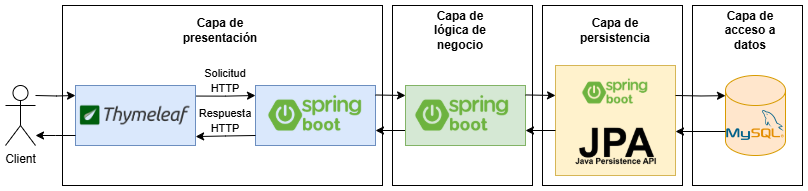
\includegraphics[width=0.95\linewidth]{imagenes//scheme/Tecnologías SIDManager.png}
    \caption{Arquitectura de las tecnologías de la aplicación SIDManager}
    \label{fig:technology_arquitecture}
\end{figure}

\section{Diagrama UML de secuencia}
Antes de desarrollar cualquier proyecto, es fundamental planificar qué se va a implementar y cómo. Por esta razón, mi tutor en la empresa me solicitaba elaborar diagramas de secuencia UML antes de trabajar en funciones clave del sistema. Estos diagramas ayudaban a visualizar el flujo de la aplicación y asegurar un diseño coherente. En este documento, se han incluido dos de los diagramas que se realizaron digitalmente: uno corresponde al proceso de registro (Figura \ref{fig:sign-up-uml-diagram}) y otro al proceso de carga de documentos filtrados por fechas (Figura \ref{fig:list-documents-uml-diagram}).


\begin{figure}
    \centering
    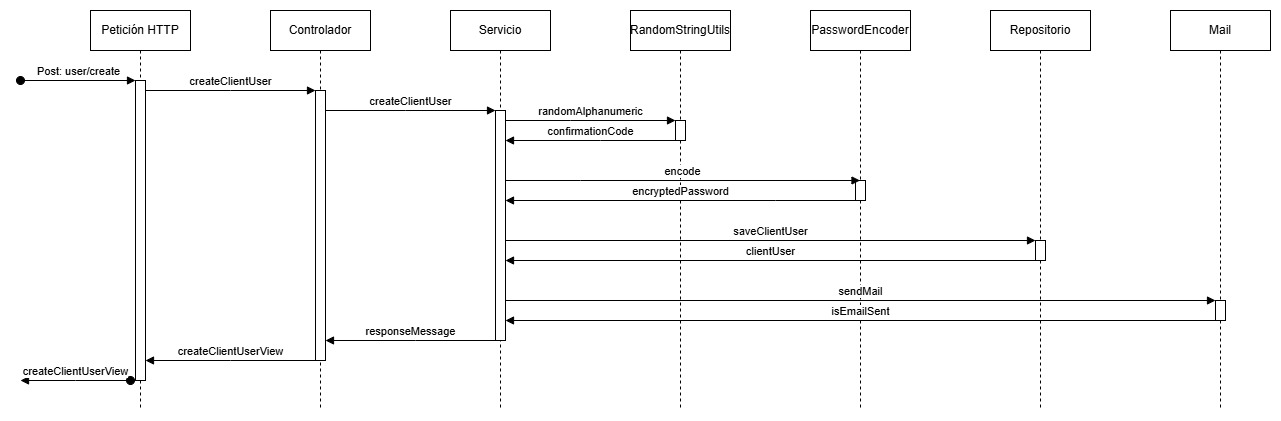
\includegraphics[width=0.95\linewidth]{imagenes/UML/SignUpPostUserCreate.jpg}
    \caption{Diagrama UML de la función createClientUser}
    \label{fig:sign-up-uml-diagram}
\end{figure}

\begin{figure}
    \centering
    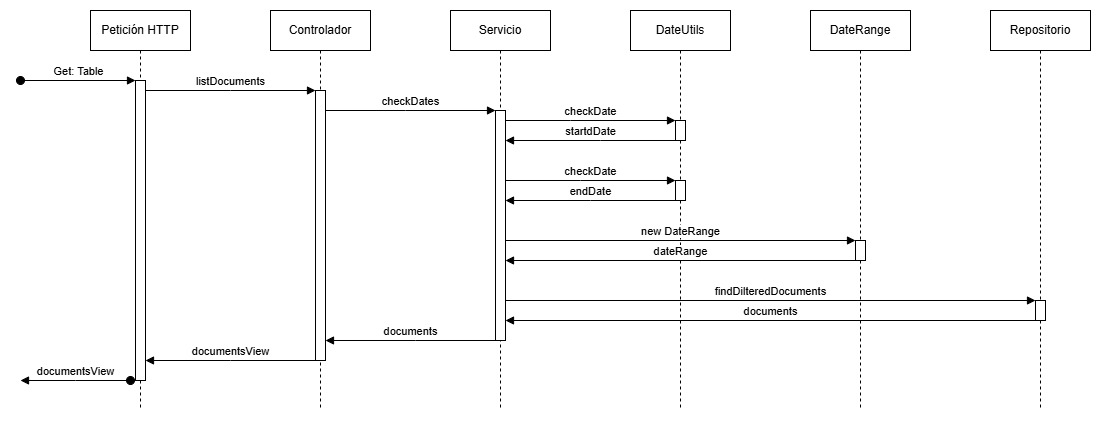
\includegraphics[width=0.95\linewidth]{imagenes/UML/getTable.jpg}
    \caption{Diagrama UML de la función listDocuments}
    \label{fig:list-documents-uml-diagram}
\end{figure}



\section{ Tecnologías selecionadas }

De las opciones de las posibles tecnologías para llevar a cabo el proyecto abordadas en el estado de la cuestión, estas son las que se han elegido:

\subsection{ Spring Boot }
Aunque existen otros frameworks populares hoy en día, como Angular y React, estos están basados en JavaScript, un lenguaje diferente de Java. JavaScript es más versátil al permitir el desarrollo tanto en frontend como en backend, pero presenta desventajas en términos de seguridad. Al no ser un lenguaje tipado ni ejecutarse en una máquina virtual, es más vulnerable a ciertos tipos de ataques, como se explica en el artículo \textcite{java-vs-javascript}. Por esta razón, para este proyecto fue necesario optar por un framework que utilizara Java.

Spring Boot ha sido la tecnología seleccionada para el desarrollo de esta aplicación web debido a sus características que facilitan la creación de aplicaciones empresariales robustas y escalables. 

Dado que el proyecto se centra en la monitorización de documentos en un entorno bancario, donde la seguridad, eficiencia y fiabilidad son aspectos clave, Spring Boot proporciona una base sólida. Con su configuración mínima y capacidades integradas, permite un desarrollo rápido y efectivo, adaptándose a las necesidades de este entorno.

Una de las principales ventajas de Spring Boot es su capacidad para simplificar el desarrollo de aplicaciones complejas gracias a su amplia gama de bibliotecas y configuraciones predeterminadas. Su integración con tecnologías como Spring Security facilita la implementación de controles de acceso y autenticación, esenciales en un entorno bancario. Además, su soporte para la gestión eficiente de bases de datos mediante JPA es ideal para manejar grandes volúmenes de datos, como los documentos almacenados en esta aplicación.

Otra ventaja importante para el uso de Spring Boot es la popularidad de Java, ya que es el séptimo lenguaje de programación más usado por profesionales según \citeauthor{most-used-tech}, como se puede ver en la figura \ref{fig:most-used-tech}. Cabe destacar en popularidad también al propio framework Spring Boot, que es el undécimo framework de desarrollo más utilizado en el mundo, como se muestra en la figura 5.2. Esto garantiza que la tecnología continúe evolucionando, lo que asegura la viabilidad del proyecto a largo plazo, además de la abundante documentación y comunidad de soporte. Spring Boot también es uno de los frameworks preferidos por los bancos, como se destaca en distintos artículos online como \textcite{java-usage-banks}. Esto se debe a su robustez, estabilidad, seguridad y escalabilidad, características clave en aplicaciones empresariales críticas.

\begin{figure}
    \centering
    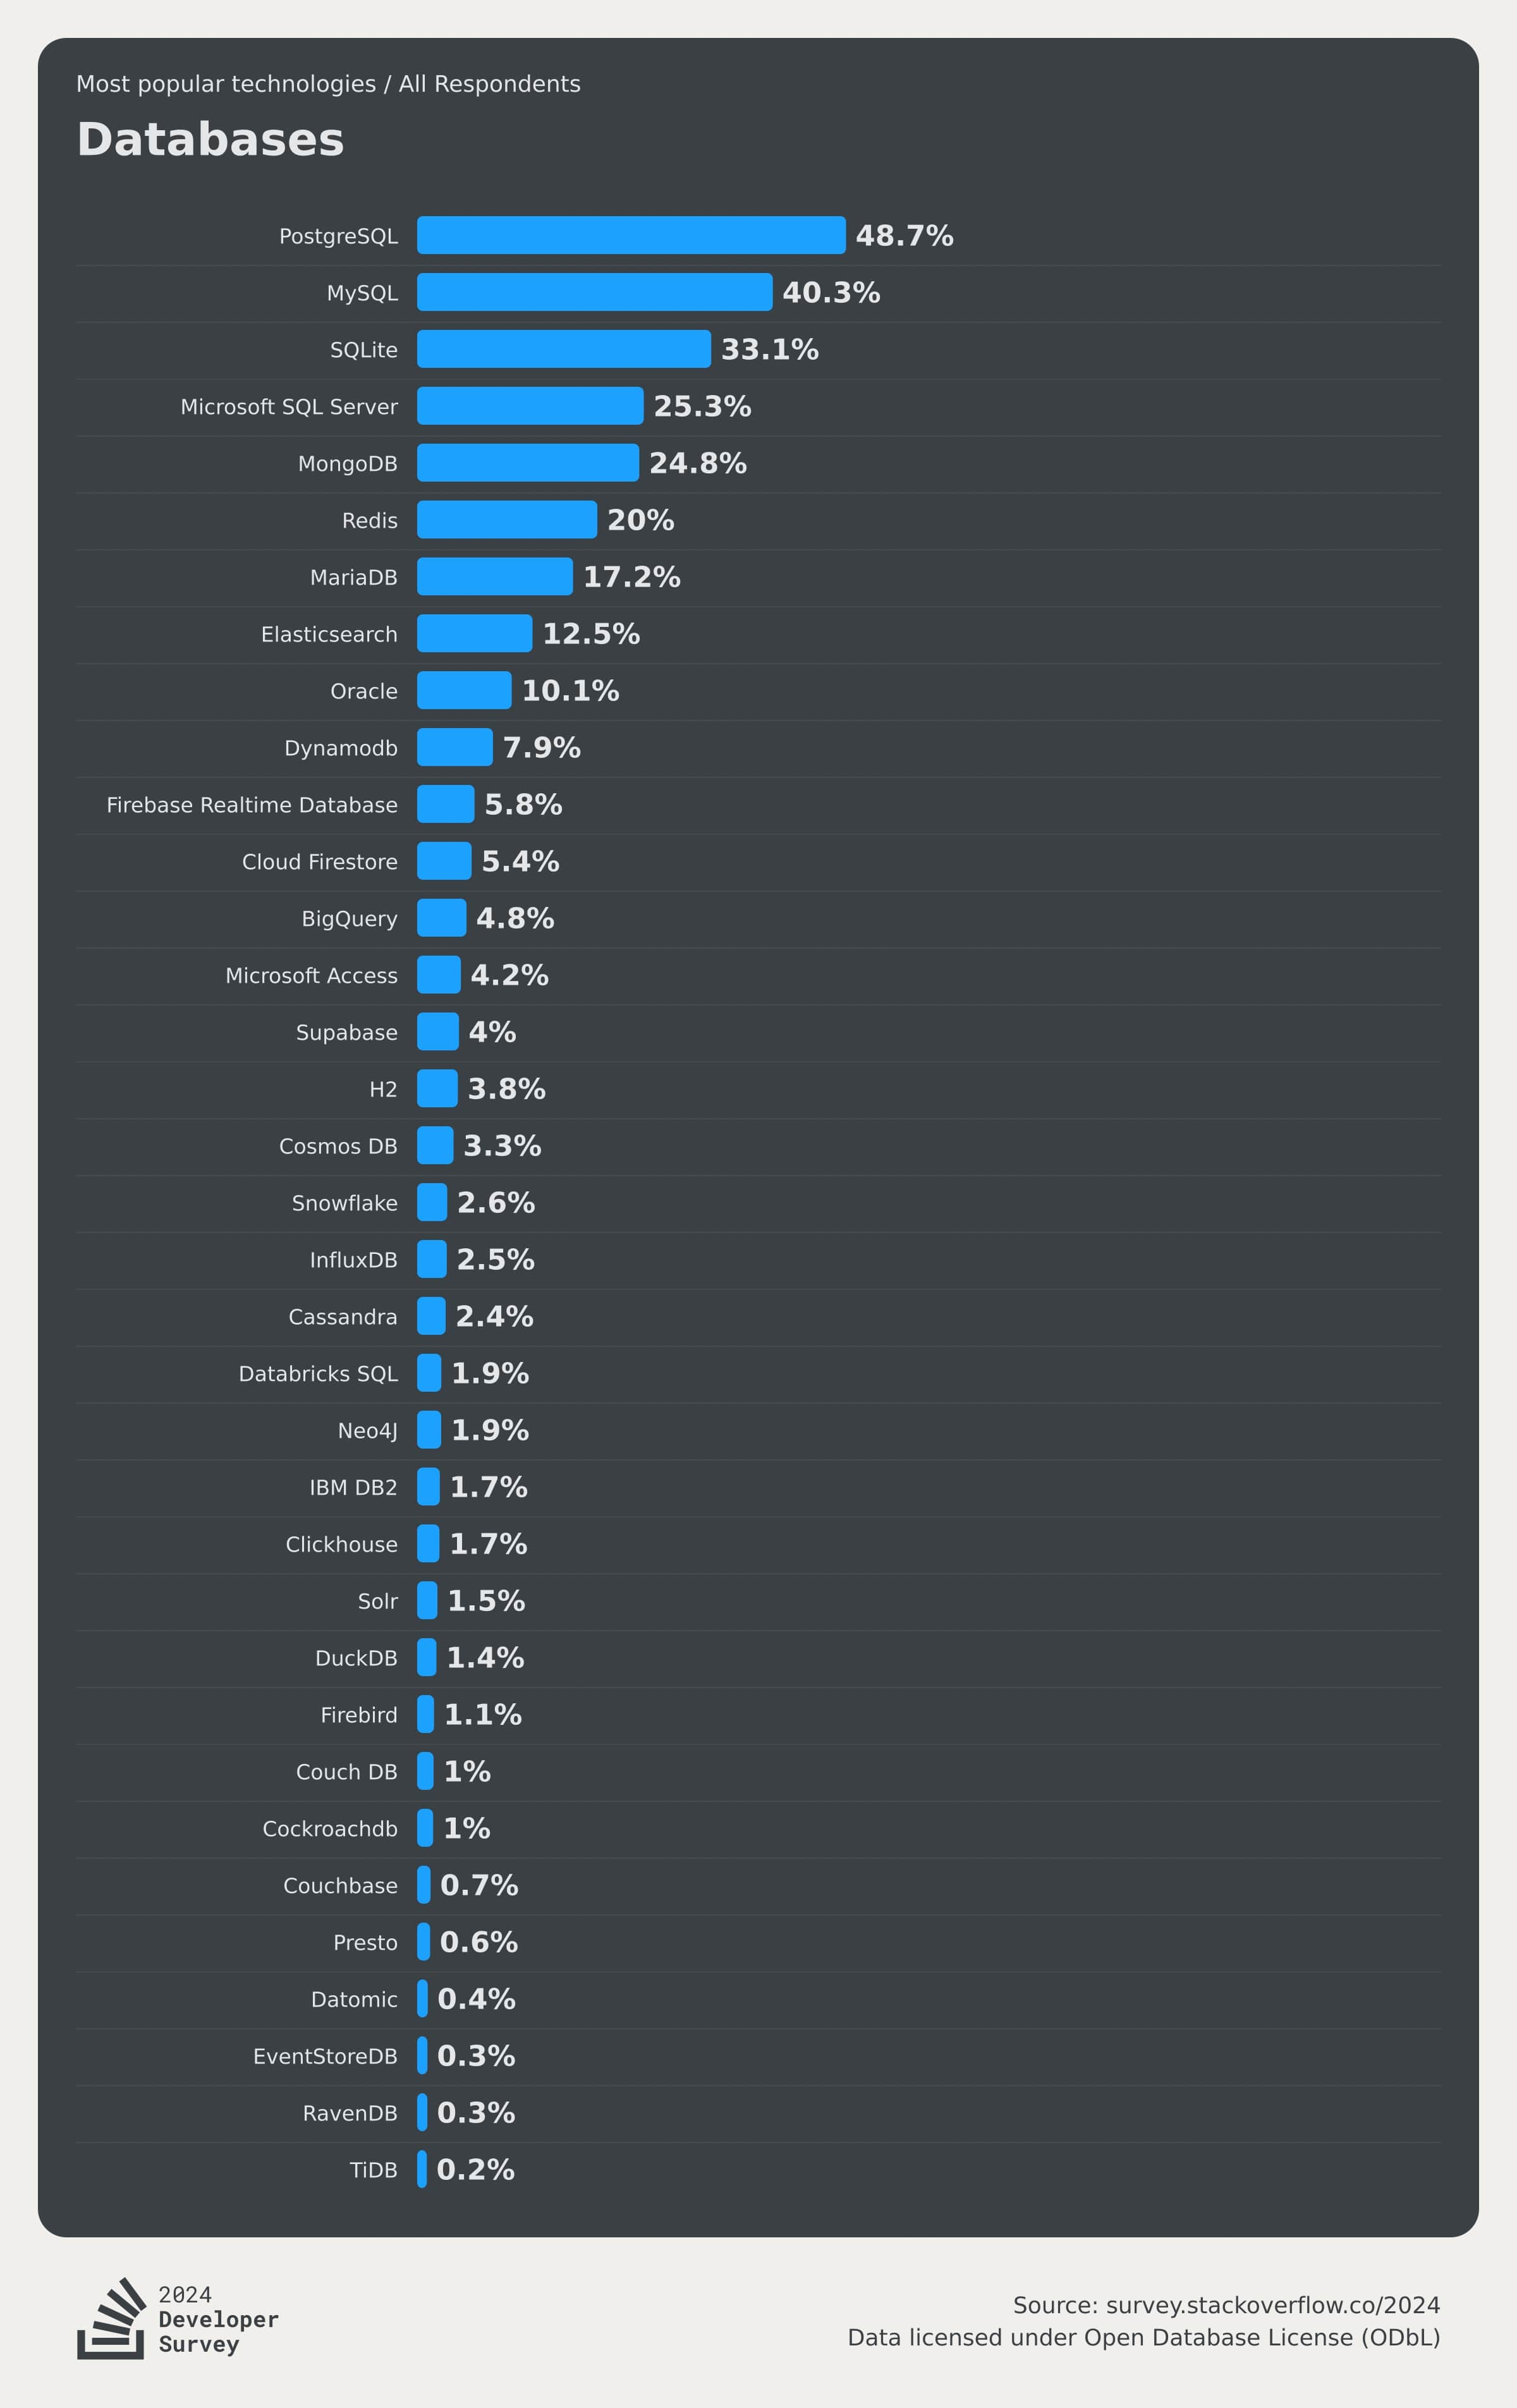
\includegraphics[width=0.85\linewidth]{imagenes/charts/java_stadistics.jpg}
    \caption{Gráfico de tecnologías más populares. Fuente: \textcite{most-used-tech}.}
    \label{fig:most-used-tech}
\end{figure}

\begin{figure}
    \centering
    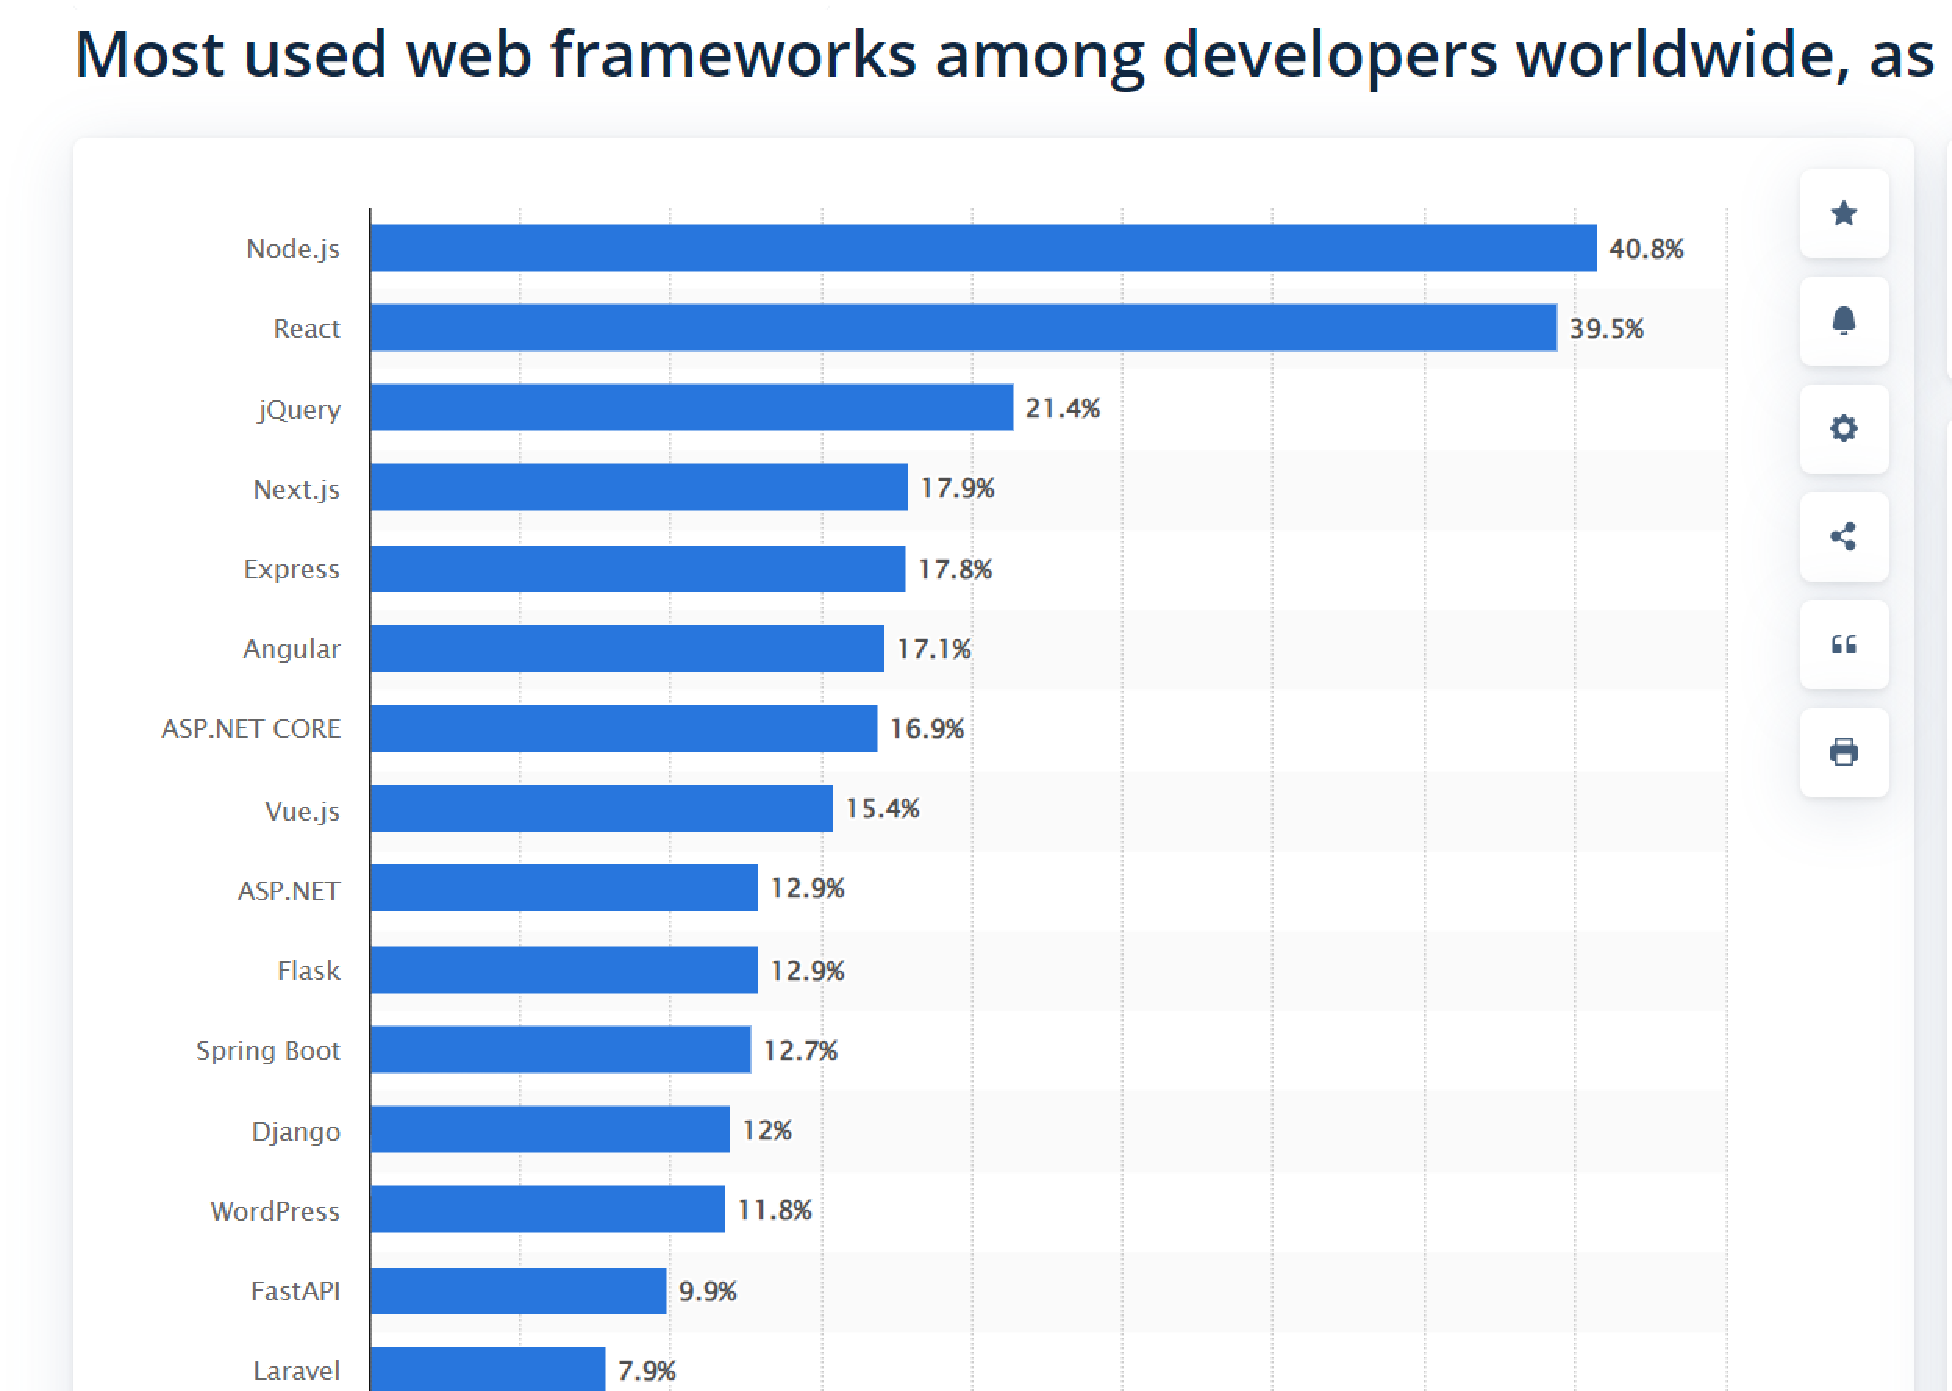
\includegraphics[width=0.9\linewidth]{imagenes/charts/spring_boot_stadistics.pdf}
    \caption{Gráfico de frameworks web más usados por desarrolladores. Fuente: \textcite{most-used-frameworks}.}
    \label{fig:most-used-frameworks}
\end{figure}



No obstante, el uso de Spring Boot también presenta ciertos inconvenientes. Aunque su automatización y configuraciones predeterminadas aceleran el desarrollo, en proyectos a gran escala pueden generar una sobrecarga del sistema si no se optimizan los recursos adecuadamente. La facilidad para incluir dependencias adicionales puede aumentar la complejidad del proyecto, afectando al rendimiento y a la mantenibilidad del código a largo plazo.

Otro aspecto a considerar es que, al estar basado en Java, Spring Boot puede requerir mayores recursos de memoria y procesamiento en comparación con tecnologías más ligeras. Esto puede ser un reto en servidores con limitaciones de hardware o cuando se buscan optimizaciones de recursos.

A pesar de estos inconvenientes, Spring Boot sigue siendo una opción sólida y flexible para desarrollar aplicaciones empresariales seguras y escalables, como es el caso de esta solución para la gestión documental en entornos bancarios.

\subsection{ Maven }

Maven ha sido elegido como la herramienta de gestión de dependencias y automatización de la construcción para este proyecto debido a su fiabilidad y popularidad en el ecosistema Java. Una de las principales razones por las que Maven es ampliamente utilizado en proyectos empresariales es su capacidad para simplificar la gestión de dependencias, lo que facilita la integración de bibliotecas externas necesarias para el correcto funcionamiento de la aplicación.

Una ventaja significativa de Maven es su capacidad para gestionar de manera eficiente las versiones de las dependencias y sus transitorios, asegurando que siempre se utilicen versiones compatibles y actualizadas de las bibliotecas, lo que es crucial para mantener la seguridad y estabilidad del proyecto en el tiempo. Además, Maven proporciona una estructura de proyecto estándar y bien organizada, lo que facilita la colaboración entre distintos equipos y la integración con herramientas de \acrfull{cicd}.

Según la encuesta de Stack Overflow, Maven es una de las herramientas de automatización de construcción más usadas en el mundo, lo que garantiza una amplia documentación y soporte por parte de la comunidad, como muestran los informes de \textcite{most-used-tech}. Esto asegura la viabilidad de su uso a largo plazo, además de la fácil capacitación de nuevos desarrolladores que se unan al proyecto.

Sin embargo, uno de los inconvenientes de Maven es su curva de aprendizaje inicial, especialmente para desarrolladores que no están familiarizados con su configuración basada en XML. Además, en proyectos de gran escala, la acumulación de dependencias puede generar archivos de configuración extensos y difíciles de manejar si no se estructuran adecuadamente. Otro aspecto a considerar es el tiempo de compilación, que puede ser considerable en proyectos grandes debido a la resolución de dependencias y la construcción de los módulos.

A pesar de estos inconvenientes, Maven sigue siendo la opción ideal para este proyecto, ya que proporciona una solución integral para la gestión de dependencias y la automatización de la construcción, permitiendo un desarrollo ágil y organizado.

\subsection{ Thymeleaf }

Thymeleaf ha sido seleccionado como el motor de plantillas para el desarrollo del frontend de esta aplicación debido a su estrecha integración con Spring Boot y su capacidad para crear vistas dinámicas basadas en HTML. Al ser una tecnología diseñada específicamente para aplicaciones web Java, Thymeleaf permite renderizar páginas de manera eficiente, con una sintaxis que resulta intuitiva para los desarrolladores que ya están familiarizados con HTML y CSS.

Una de las principales ventajas de Thymeleaf es que permite construir plantillas que son directamente visualizables en navegadores, incluso sin un servidor backend activo, lo que agiliza el desarrollo de interfaces. Esto se alinea con la necesidad de este proyecto de desarrollar una aplicación web accesible y fácil de mantener. Además, Thymeleaf soporta la validación de formularios y la internacionalización, características clave para una aplicación que pueda ser utilizada en distintos contextos empresariales y por usuarios de diversas regiones.

Según la propia web de \citeauthor{thymeleaf-downloads}, es uno de los motores de plantillas más populares dentro del ecosistema de Spring, ya que tiene más de un millón y medio de descargas al mes, lo que asegura la existencia de abundante documentación y ejemplos prácticos, como se puede ver en el siguiente gráfico \ref{fig:descargas_mensuales_thymeleaf}. Esto facilita su integración y reduce la curva de aprendizaje para nuevos desarrolladores.

\begin{figure}
    \centering
    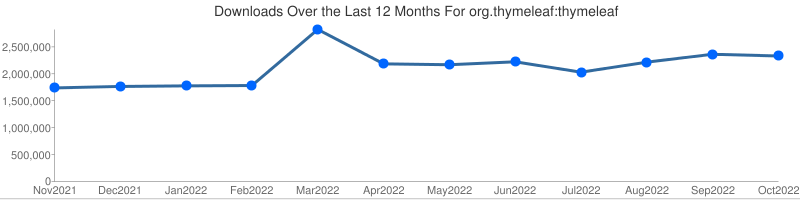
\includegraphics[width=0.75\linewidth]{imagenes/charts/thymeleaf_usage.png}
    \caption{Descargas mensuales de Thymeleaf. Fuente: \textcite{thymeleaf-downloads}.}
    \label{fig:descargas_mensuales_thymeleaf}
\end{figure}

No obstante, Thymeleaf presenta algunos inconvenientes. Al ser un motor de plantillas del lado del servidor, puede tener un rendimiento inferior en comparación con soluciones de frontend basadas en JavaScript, como React o Angular, especialmente cuando se trata de aplicaciones con una gran cantidad de interacciones simultáneas. Además, la generación de vistas en el servidor puede aumentar la carga de procesamiento en aplicaciones con un gran número de usuarios concurrentes, lo que puede requerir optimizaciones adicionales en el backend.

A pesar de estos desafíos, Thymeleaf sigue siendo una opción adecuada para este proyecto, ya que facilita la creación de una interfaz de usuario dinámica y bien integrada con Spring Boot, manteniendo un enfoque en la simplicidad y la seguridad, lo cual es crucial para aplicaciones bancarias y empresariales.


\subsection{ JPA }

JPA (Java Persistence API) ha sido elegido en este proyecto por su capacidad para simplificar la interacción con la base de datos, eliminando la necesidad de escribir consultas SQL manuales en la mayoría de los casos. Al trabajar con JPA, el desarrollador puede centrarse en los objetos de dominio de Java, ya que JPA se encarga de la persistencia de los datos de manera automática, permitiendo asignar las entidades directamente a las tablas de la base de datos.

Una de las principales ventajas de JPA es su capacidad para abstraer la complejidad del SQL. Esto simplifica el desarrollo al utilizar operaciones CRUD predefinidas y un lenguaje de consultas más amigable como \acrfull{jpql}, que evita la necesidad de escribir SQL detallado. Además, JPA se integra perfectamente con Spring Data, lo que permite generar repositorios y consultas dinámicas de forma automática, lo cual mejora la productividad y reduce el riesgo de errores en la interacción con la base de datos.

\begin{figure}
    \centering
    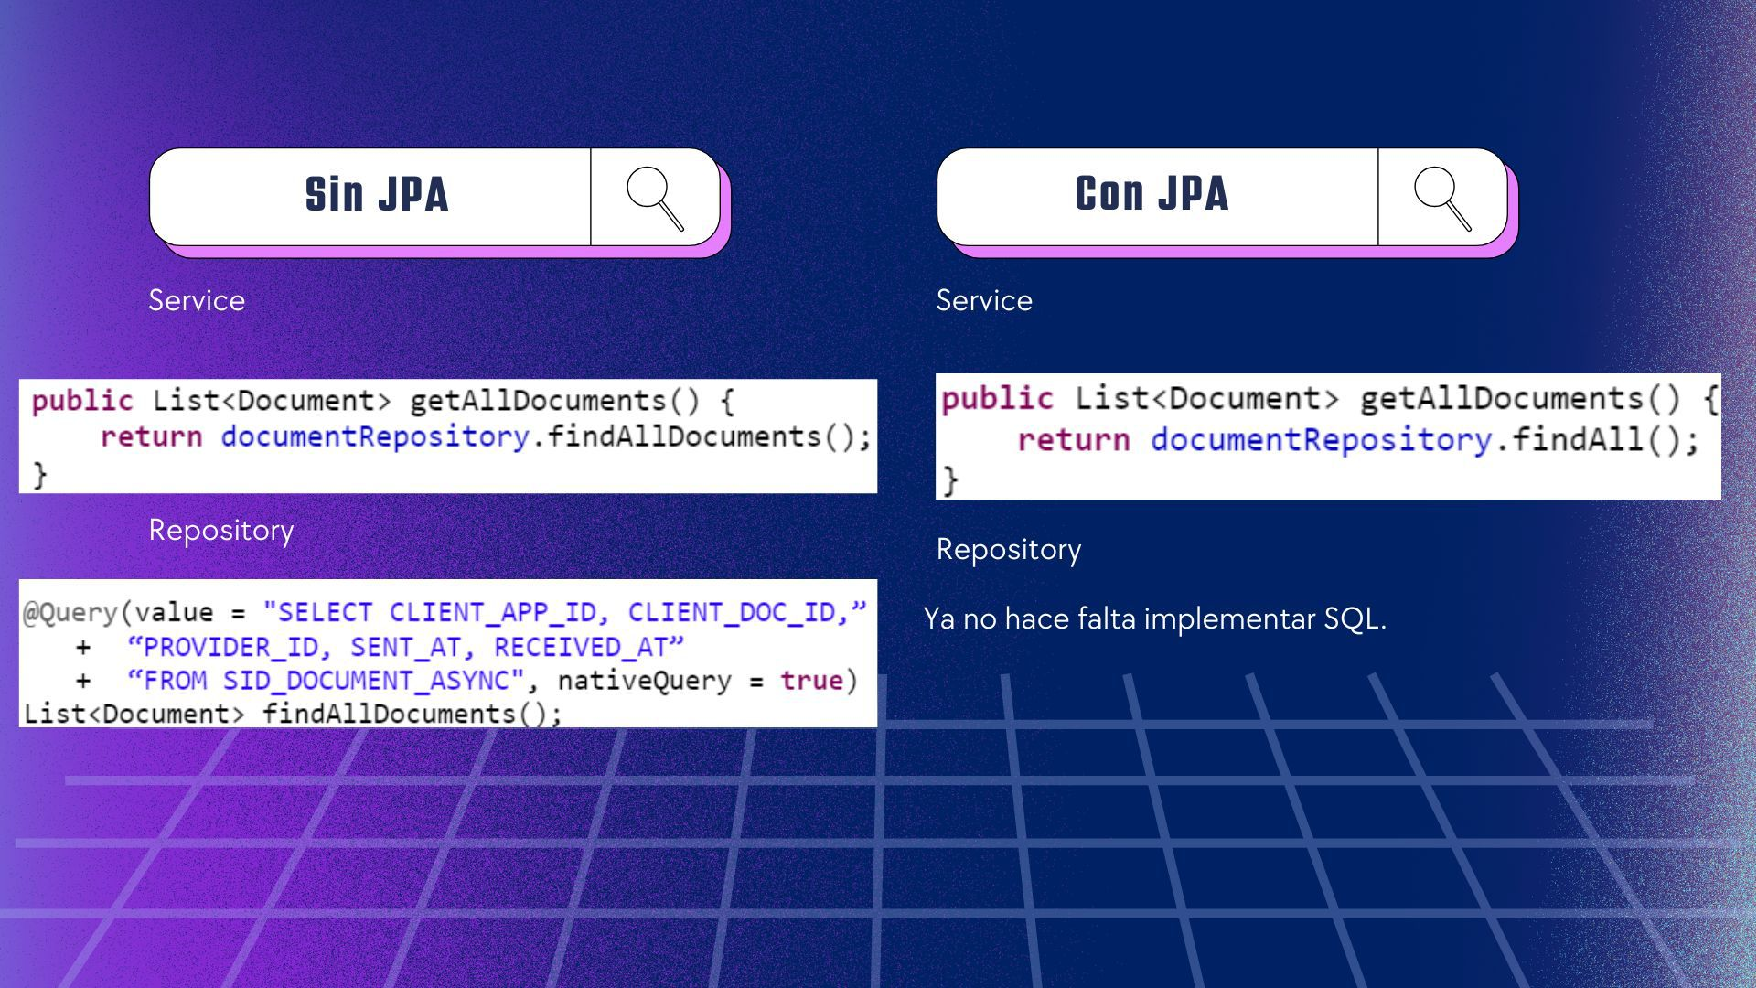
\includegraphics[width=0.75\linewidth]{imagenes/code/JPA_usage.pdf}
    \caption{Diferencia entre usar y no usar JPA (elaboración propia).}
    \label{fig:jpa-usage}
\end{figure}

JPA también garantiza la independencia de la base de datos, ya que facilita la migración entre distintos sistemas de gestión de bases de datos sin cambios significativos en el código. 

Sin embargo, uno de los inconvenientes de JPA es su rendimiento en escenarios con consultas SQL muy complejas o específicas, donde puede ser necesario optimizar manualmente el SQL para obtener mejores tiempos de respuesta. Además, JPA puede añadir una cierta sobrecarga en términos de recursos debido a la gestión de la caché y las transacciones automáticas.

A pesar de estos desafíos, JPA sigue siendo una opción ideal para este proyecto, ya que facilita enormemente la gestión de la persistencia de datos, minimizando la necesidad de escribir SQL manual y aumentando la eficiencia del desarrollo.
